
\section{Method}\label{method}
This chapter provides a clear and extensive description of the methodology undertaken to address the question the thesis is based on. The intention is to enable the methodology to be reproducible. This is accomplished by dividing the method into several steps and for each one describing the processes they involve, the tools used, and criteria for completion.
 
\subsection{Structure}\label{structure}

To answer the question if formal specifications can be used during porting processes, the methodology was divided into discrete steps (see figure \ref{fig:vmodel}).
The steps and their ordering can be compared to the V-model; a widely adopted software development project model \cite{VEEMODEL}. The V-model describes a procedure, where high-level requirements are assembled first and then as the process goes on, the detail level is increased until implementation. The model also describes verification stages corresponding to each of these previous stages. The verification begins with the smallest granularity of tests and becomes more high-level until finally acceptance testing is performed. The methodology described in this thesis, can be seen as an inversion of the V-model where the process starts already having an original source. By writing tests, the behavior of the original was ascertained. On the highest abstraction level, the model specification lives. This represents the high-level requirements of the traditional V-model. The last verification step exists as a bridge between the original source and the ported source. Figure \ref{fig:vmodel} shows a minimal representation of the V-model, and how this process can be seen as an inversion of it.   

\begin{figure}[H]
\centerline{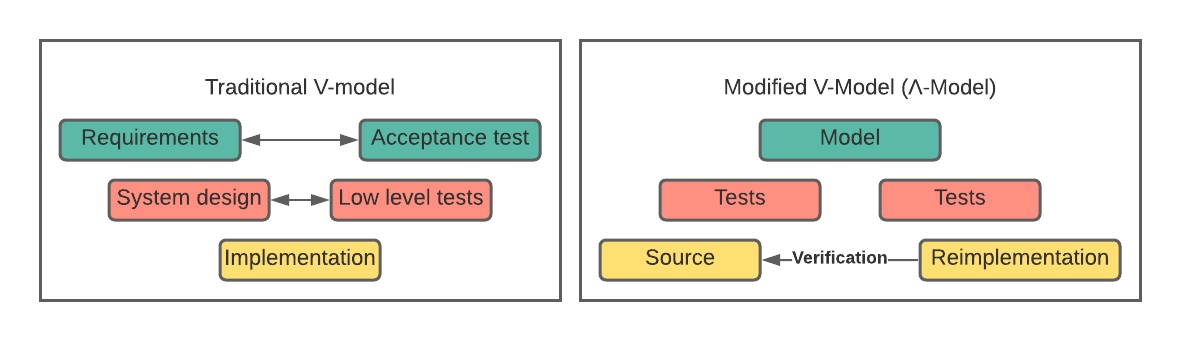
\includegraphics[width=5in]{V-model_.png}}
\caption{Simplified V-model of Software Development, Alongside a Modified Version of the Model}
\label{fig:vmodel}
\end{figure}
\newpage
To get a more detailed description of the method, it was divided into the following steps: 

\begin{enumerate}
  \item Find an established and well used open-source library as a target source code.
  \item Select a suitable testing framework and implement tests on the target source code to form an understanding of its behaviors and functionalities.
  \item Find a formal specification language and reverse engineer the target source code by creating a model of it. This model is to be derived from the tests implemented in the previous step.
  \item Implement tests for the functionalities specified in the created model.
  \item Implement the functionalities in the target language based on the tests created.
  \item Verify that the implementation is a true port of the target source code using a verification test-suite. The test-suite should run on both the original compiled code and a compiled version of the new implementation without modification.
\end{enumerate}



\subsection{Testing}\label{tests}

For this thesis, testing was performed to create an understanding of the system under test. This is a reversal of the traditional role of the test code. To select tools and metrics that fitted this purpose best, constraints that applied to this specific scenario were considered. The tests needed to be able to verify to such a degree that all the behaviors of the code were accounted for. For example, there could have been some scenario which yielded unintuitive results; some behavior that did not match the porting parties' expectations. It was important to find these cases, not to expose them to fix, but to build a complete understanding of what the code did. 

To achieve this in as an efficient manner as possible, the test-methodology chosen for the thesis fell on property-based testing. This practice entails that the test code describes some operation that is permissible to the system under test along with the constraints on the input data for that operation (see section \ref{pbtesting}). This approach was assumed to be particularly useful for this endeavor because it can be utilized without knowing the intentions of the system under test and can be seen as a guided exploration on the test subject rather than verification.

Like most data structures, the subject of the port will likely have some state which may or may not be permuted by the available operations. To make sure that the tests fully exercise this property of the code, and that the assumptions made also hold true over the lifetime of the system, a stateful test-suite was also created (see section \ref{pbtesting}). This meant that some operations and predicates which determine when the operation is valid were defined, along with a model. 

To perform all these tests, a test framework was used. A test-framework provides a convenience in the test-writing process, foremost since it provides some code to drive the tests - code often referred to as a test runner. This frees the developer from the burden of verifying that all tests are run, as well as collecting statistics and logging failures. To determine when tests were sufficient, the metric of test-coverage by branch and line-of-code was used. That way it was easy to verify that each branch, and/or line had been exercised. There were, therefore, some requirements that a chosen framework had to fulfill to satisfy the needs of the project.

\subsubsection{Frameworks}

The choice of frameworks fell on GoogleTest \cite{GOOGLETEST} as it was a widely adopted unit testing library. It also allowed tests to be written in C++ which enabled the subject to be easily tested with minimal modification. RapidCheck \cite{RAPIDCHECK} was chosen as a framework for the property-based testing since it was easy to use alongside GoogleTest; RapidCheck allows for specification of properties in an imperative style which works well for C++. 


\subsubsection{Environment}\label{environment}

To execute tests on the C source code, a test environment needed to be set up. The project and dependencies were acquired and built automatically using CMake \cite{CMAKE} which is an easy-to-use tool for automating these types of procedures. As an IDE, CLion \cite{CLION} was chosen as it is a cross-platform IDE for C and C++. CLion also provides integration with CMake, allowing for a simple build procedure. The GNU C++ compiler g++ was used to compile the source code \cite{GCC}.

\newpage

\subsubsection{Implementation Process}\label{implproc}

The initial intention was to create tests in a methodical and structured way. To accomplish this, these steps of deductive reasoning and test implementations, inspired by Hoare logic (see section \ref{hoare}), were created and followed:

\begin{enumerate}
  \item Select a functionality to write tests for.
  \item Provide a logical basis for the program properties. This should be done by making several assertions on the functions precondition as well as on the results obtained on termination i.e., the values which the relevant variables will take before and after execution of the program. 
  \item Create tests based on the logical basis to see if the program is understood correctly and carries out the functionalities identified.
  \item Modify tests to match any discrepancies found between actual and expected behavior.
  \item Repeat all steps until all functionality of importance has been identified and tested.
\end{enumerate}


\subsection{Reimplementation}\label{reimpl}
A TDD methodology was the approach chosen when implementing the formal model into Rust code, interleaving writing the tests with the actual implementation. The TDD used in this project followed the steps defined in figure \ref{fig:testdriven}, with the addition that new functionalities are found only from the model, by one of its invariants. The tests should be written so that when they pass, an invariant - or part of one - should be fulfilled. The fact that the tests are based on the model - and TDD's self-documenting nature - should make explicit the relation between the model and the implementation.

\subsection{Verification}\label{verification}

With the ported code in place, it should behave the same way as the original. To verify this, the port and source were both built as linkable libraries sharing the same application programming interface (API) allowing them to be tested by one single set of tests (see figure \ref{fig:api}). This made it possible to swap out the system-under-test without changing the test-code, thereby serving as an independent verification that the two implementations behaves the same. This can be compared to how hardware components can be tested in a single test-bed and quickly swapped out for the next component.

This verification process requires that the source and target language have interoperability with, and can be called by some common language, preferably the one used to write the original tests (see section \ref{implproc}). In the case of this project - where C and Rust were the languages used - interoperability can be achieved by creating a foreign function interface (FFI) by declaring matching external functions that call the appropriate library functions. 

\begin{figure}[H]
\centerline{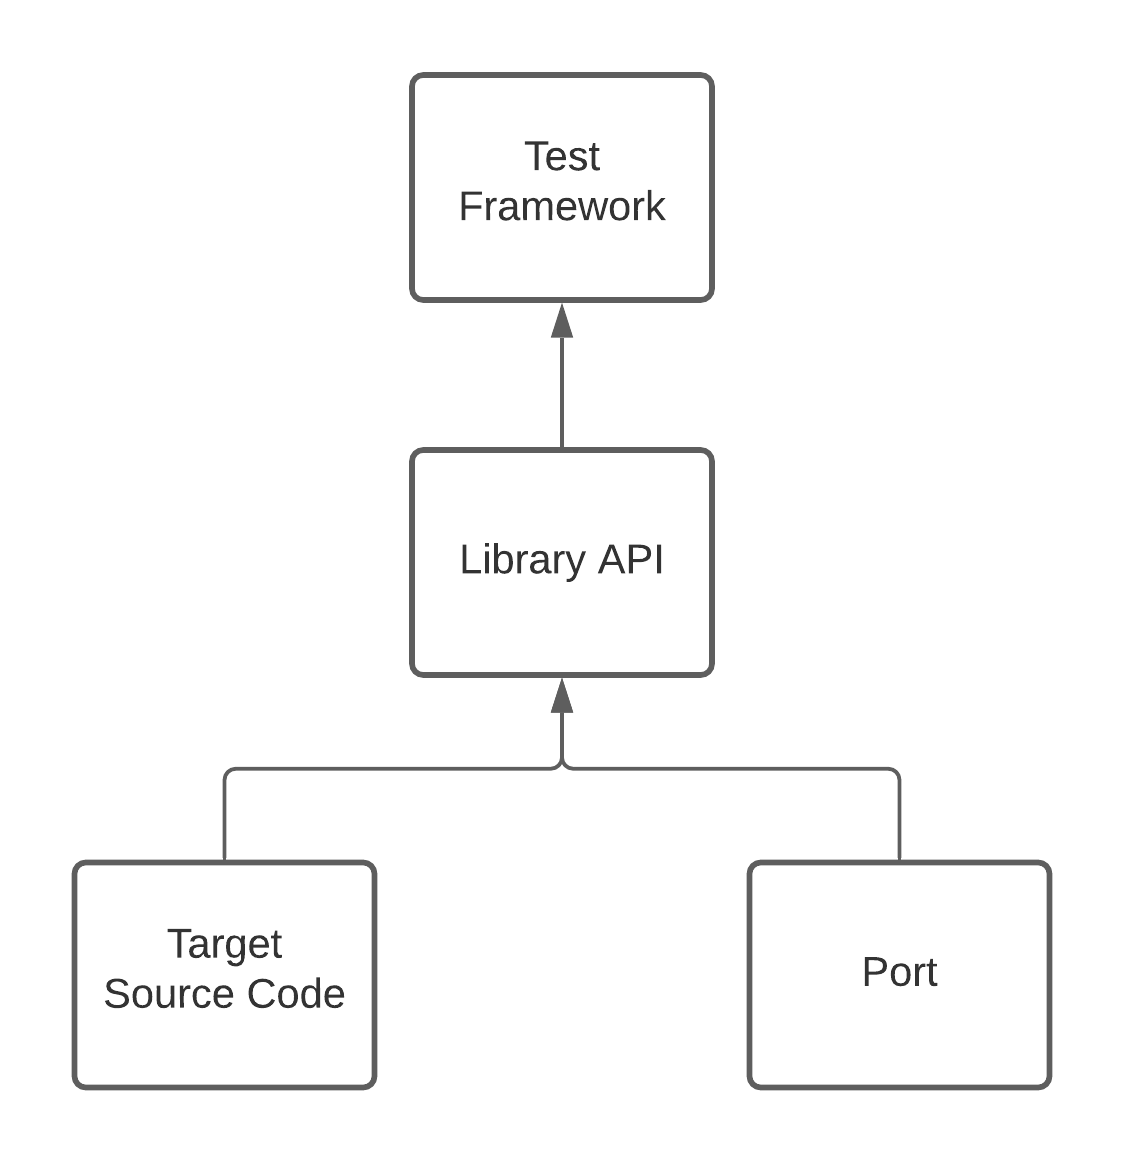
\includegraphics[width=2.5in]{api.png}}
\caption{Verification Structure}
\label{fig:api}
\end{figure}

As well as serving as the final evaluation of the final product, whether this last step is successful also serves as an evaluation of the method proposed. If it is successful then it can be concluded that this method is a feasible way of porting software. There is one caveat to this last step of the method process, knowing some of the differences between C and Rust. While the intention is to leave the original library as unmodified as possible, it may be necessary - or at least convenient - to insert one or a few helper functions into the library version of the source that manages the creation of lists etc. This will likely aid in keeping the interfaces to the libraries identical, while allowing the ported code to be more Rust “idiomatic”. The key to the success of this type of verification process will be to not add functionality influencing the test results, and consequently invalidating the conclusion of the tests.